\section{Resultados}
En esta sección incluiremos los resultados de la experimentación que realizamos con las redes desarrolladas.\\

La idea general de los experimentos es intentar medir la performance
de cada red observando, en el primer problema, la distribución espacial de los clusters de empresas y en el segundo, la calidad 
del mapa generado.\\

Presentamos en primer lugar los resultados obtenidos del problema de reducción de dimensiones.

\subsection{Ejercicio 1 - Reducción de dimensiones}

Para el primer ejercicio, los experimentos consistieron en variar la cantidad de épocas, la regla de aprendizaje y la cantidad de dimensiones de salida. Intentamos variar estos factores y observar diferencias en los gráficos 3D generados en base a las nuevas dimensiones.\\

Comenzamos realizando clasificaciones con 100 épocas. Al obtener resultados imprecisos subimos la cantidad a 200. Allí observamos una clasificación mejor, más marcada la separación geométrica entre los distintos clusters.\\

Luego comparamos los resultados obtenidos entre las distintas reglas. Repetimos las ejecuciones variando la regla entre Oja y Sanger para comprobar su eficacia.\\

Por último, decidimos cambiar la cantidad de dimensiones de sálida, esperando una mejora en las clasificaciones. 

\subsubsection{Regla de Oja - 200 épocas}
En los primeros experimentos, fuimos probando la calidad de la clasificación utilizando solamente 100 épocas. La decisión se basó en un tema de performance de la red. Cada ejecución tenía una cierta demora, por lo que empezamos probando con pocas épocas. Mostramos los primeros resultados que obtuvimos, utilizando la regla de Oja:

\begin{figure}[h]
  \begin{center}
    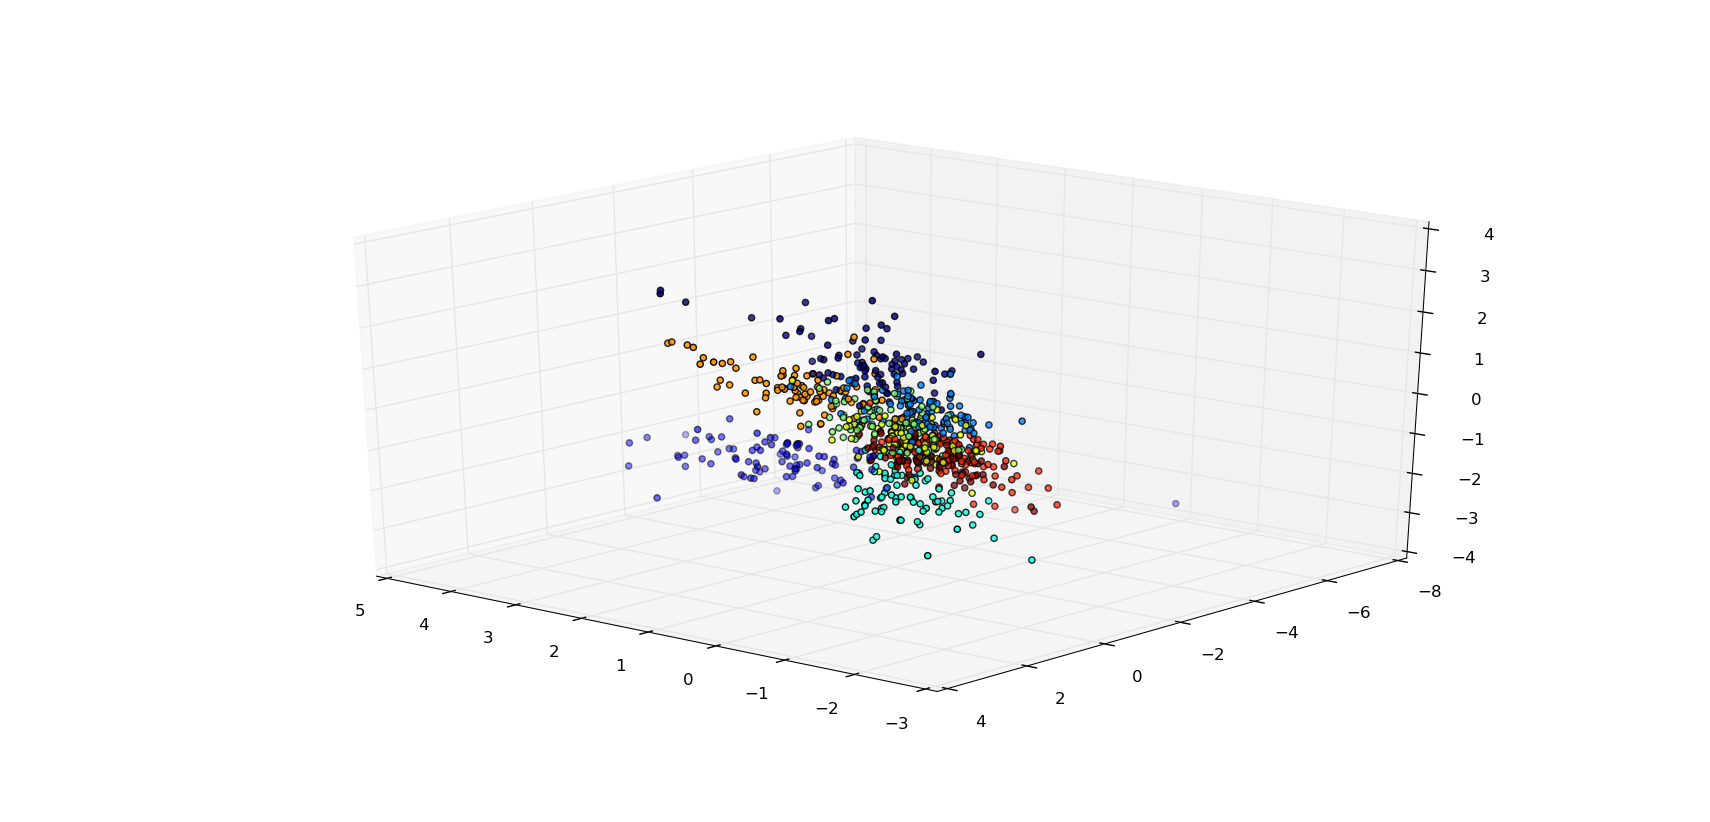
\includegraphics[scale=0.4]{../img/ej1/oja/alt-oja_3salida_200ep_train.png}
  \caption{Oja - 3 dimensiones - 200 épocas - Datos Entrenamiento}
  \end{center}
\end{figure}

\begin{figure}[h]
  \begin{center}
    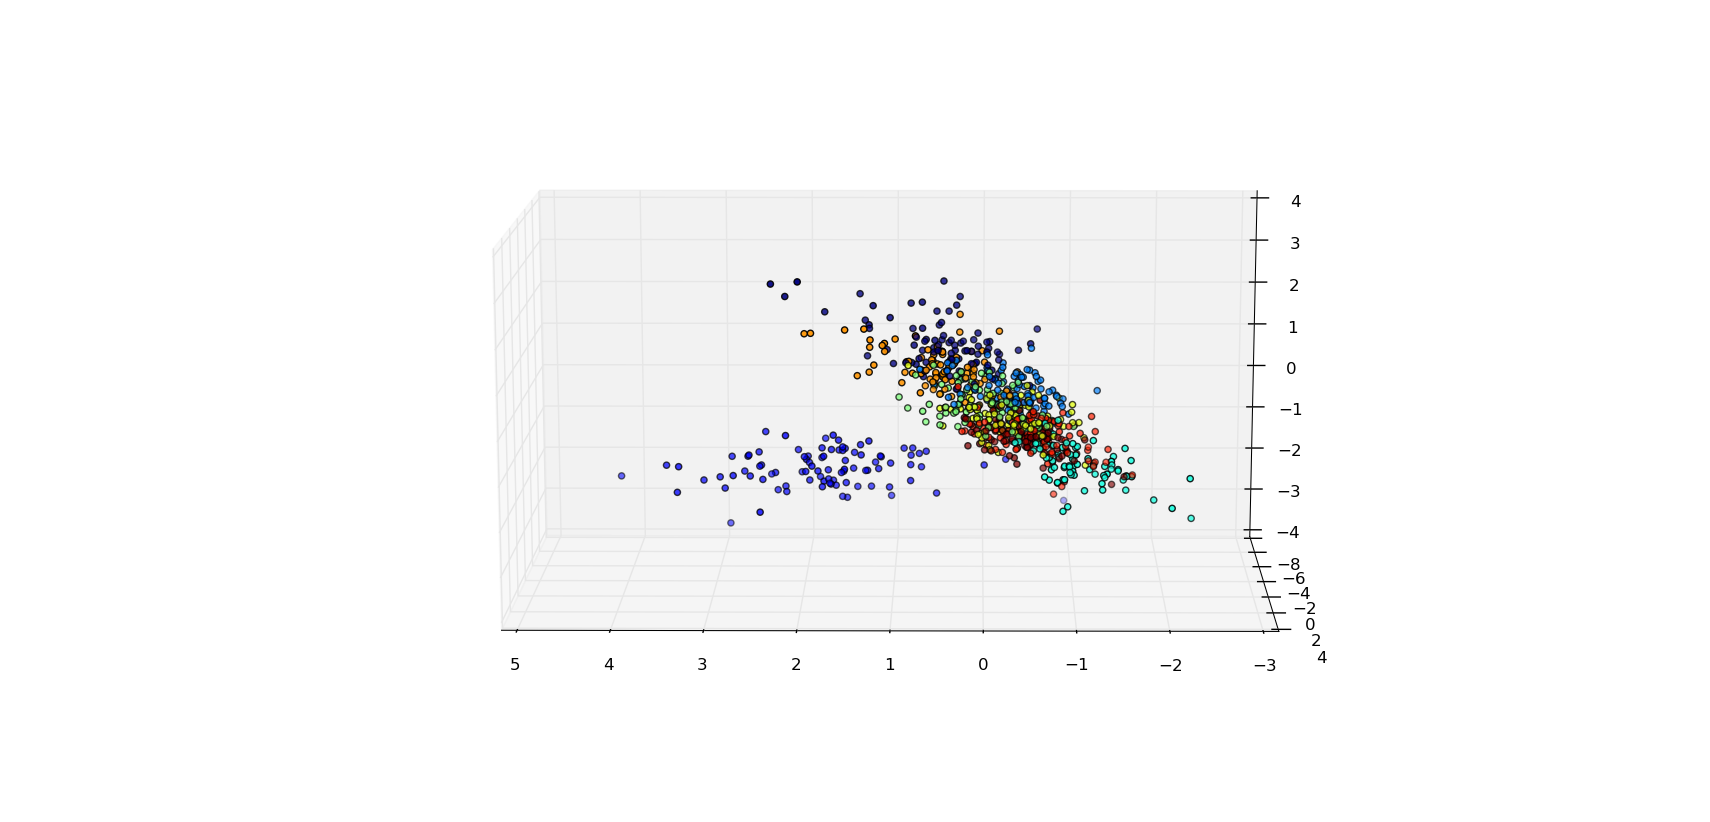
\includegraphics[scale=0.4]{../img/ej1/oja/alt-oja_3salida_200ep_train_2.png}
  \caption{Oja - 3 dimensiones - 200 épocas - Datos Entrenamiento}
  \end{center}
\end{figure}

\begin{figure}[h]
  \begin{center}
    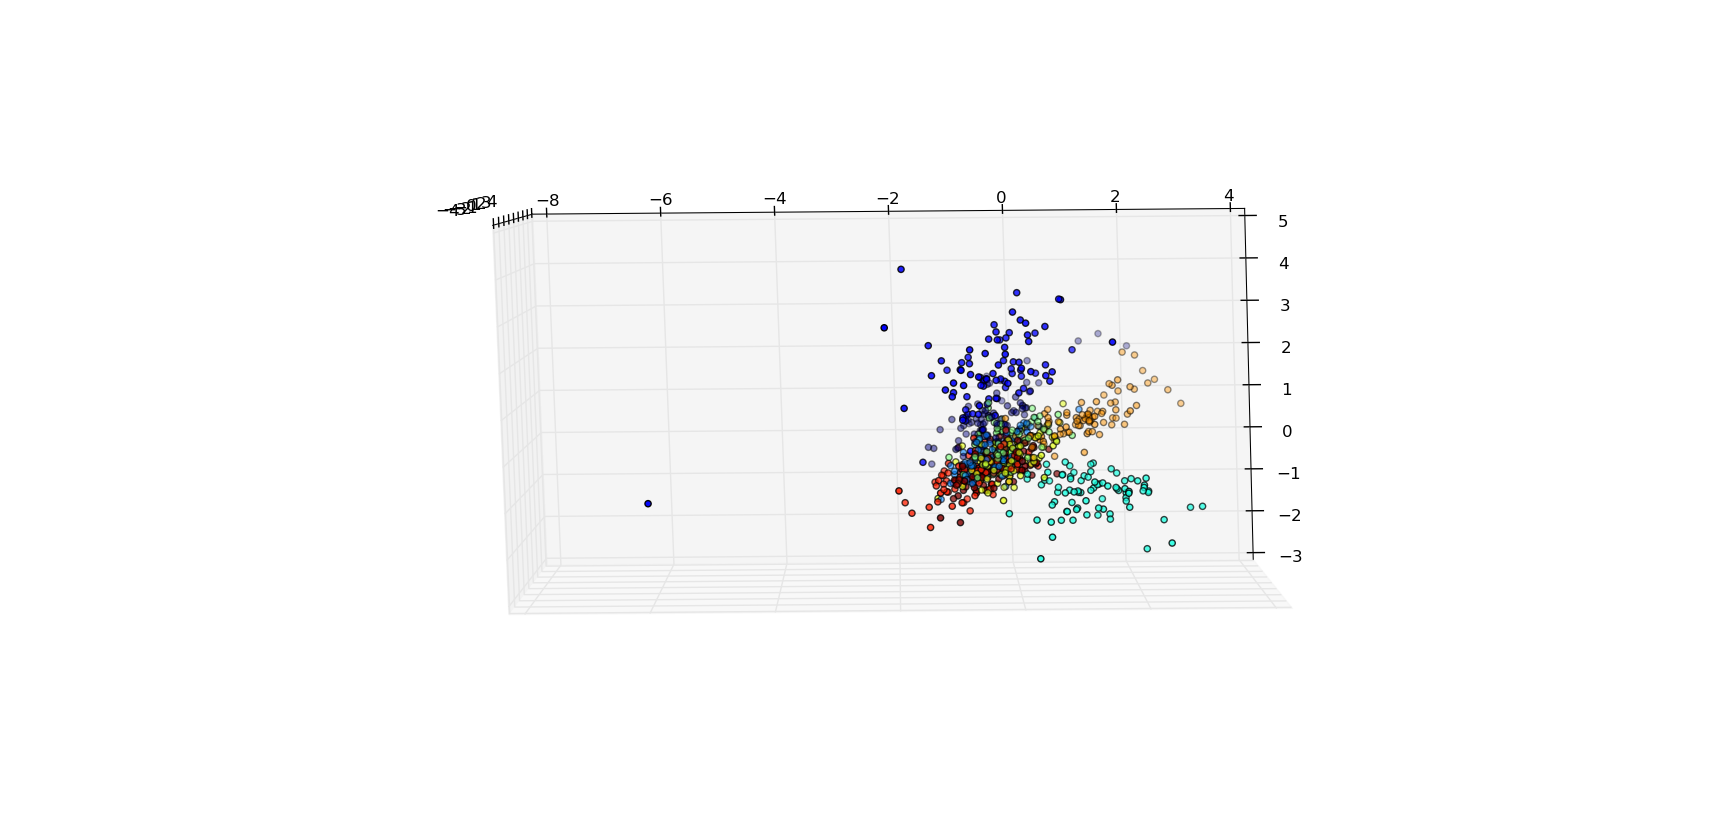
\includegraphics[scale=0.4]{../img/ej1/oja/alt-oja_3salida_200ep_train_3.png}
  \caption{Oja - 3 dimensiones - 200 épocas - Datos Entrenamiento}
  \end{center}
\end{figure}

\begin{figure}[h]
  \begin{center}
    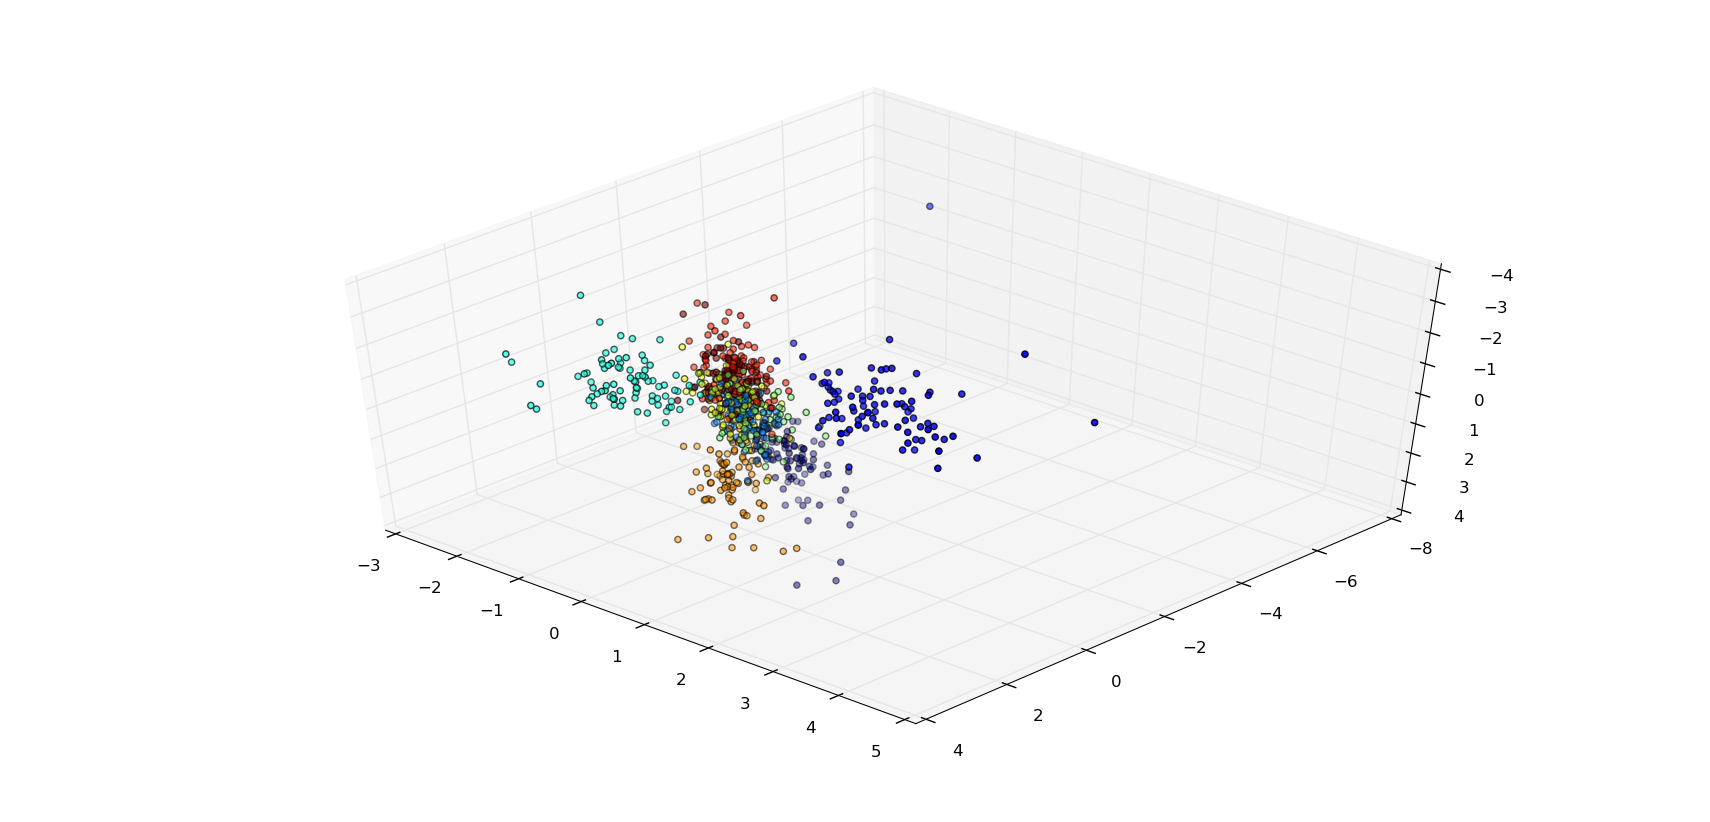
\includegraphics[scale=0.4]{../img/ej1/oja/alt-oja_3salida_200ep_train_4.png}
  \caption{Oja - 3 dimensiones - 200 épocas - Datos Entrenamiento}
  \end{center}
\end{figure}

\begin{figure}[h]
  \begin{center}
    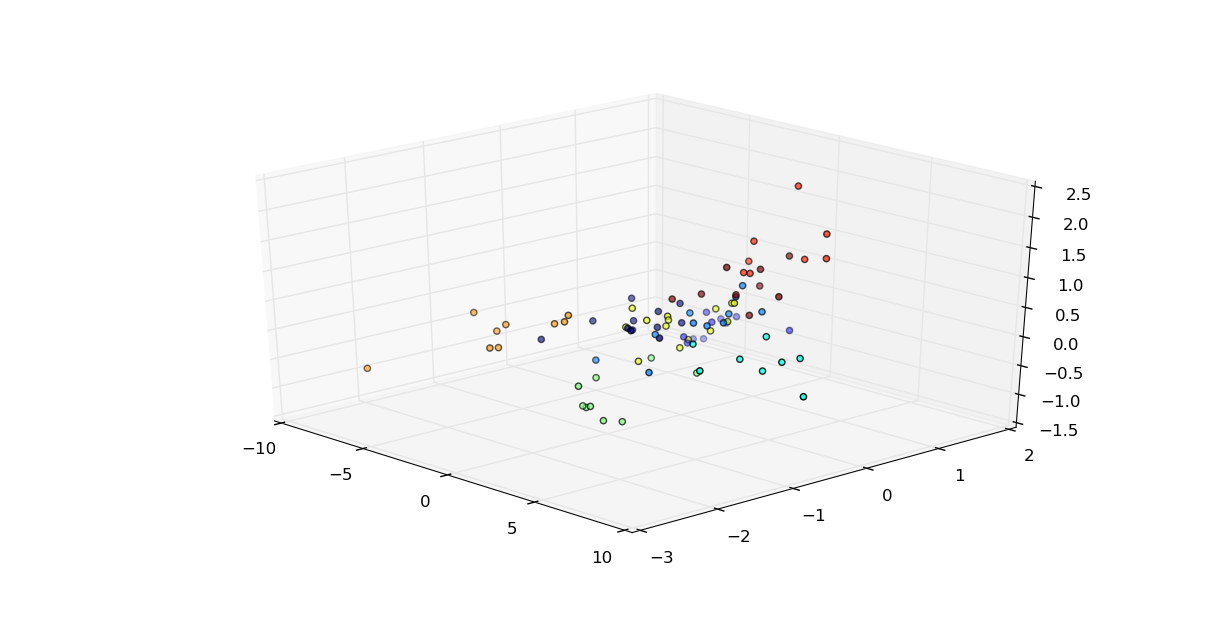
\includegraphics[scale=0.6]{../img/ej1/oja/alt-oja_3salida_200ep_validation.png}
  \caption{Oja - 3 dimensiones - 200 épocas - Datos Validación}
  \end{center}
\end{figure}

\begin{figure}[h]
  \begin{center}
    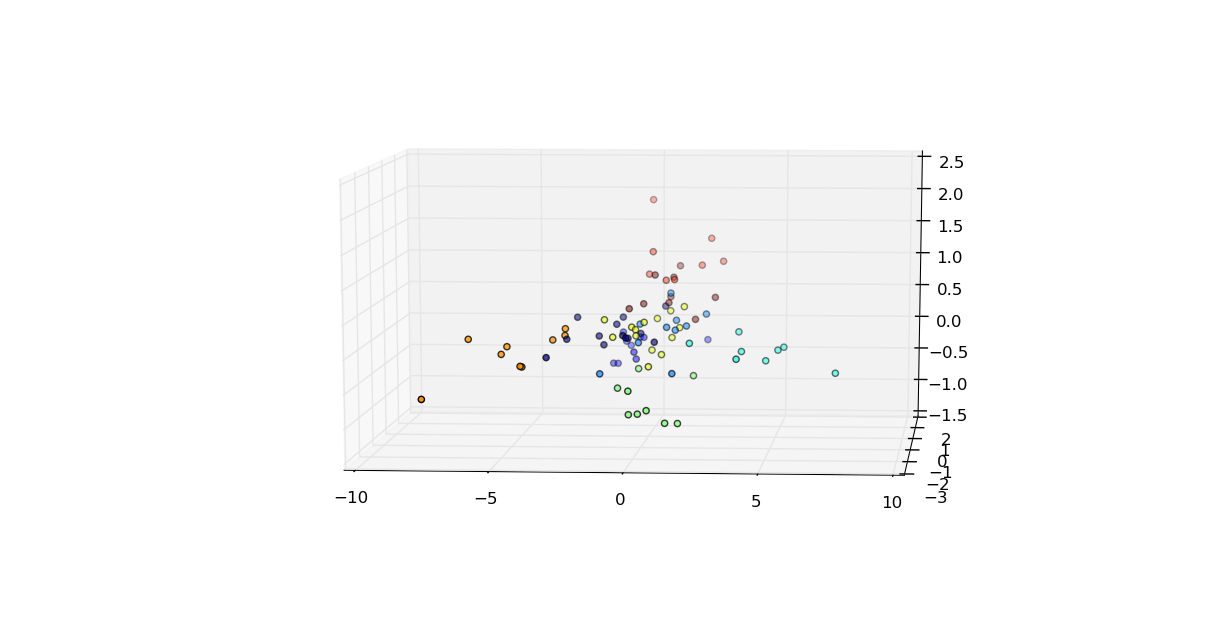
\includegraphics[scale=0.6]{../img/ej1/oja/alt-oja_3salida_200ep_validation_2.png}
  \caption{Oja - 3 dimensiones - 200 épocas - Datos Validación}
  \end{center}
\end{figure}

\begin{figure}[h]
  \begin{center}
    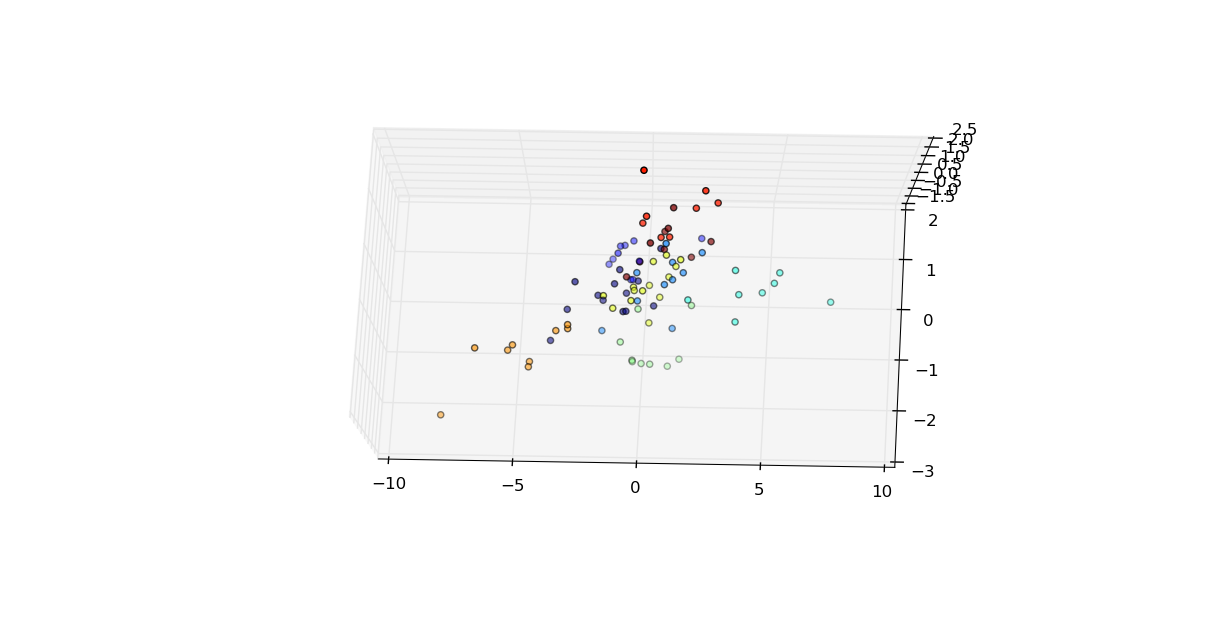
\includegraphics[scale=0.6]{../img/ej1/oja/alt-oja_3salida_200ep_validation_3.png}
  \caption{Oja - 3 dimensiones - 200 épocas - Datos Validación}
  \end{center}
\end{figure}
% \begin{figure}[!htbp]
% \centering
% \begin{subfigure}{.5\textwidth}
%   \centering
%   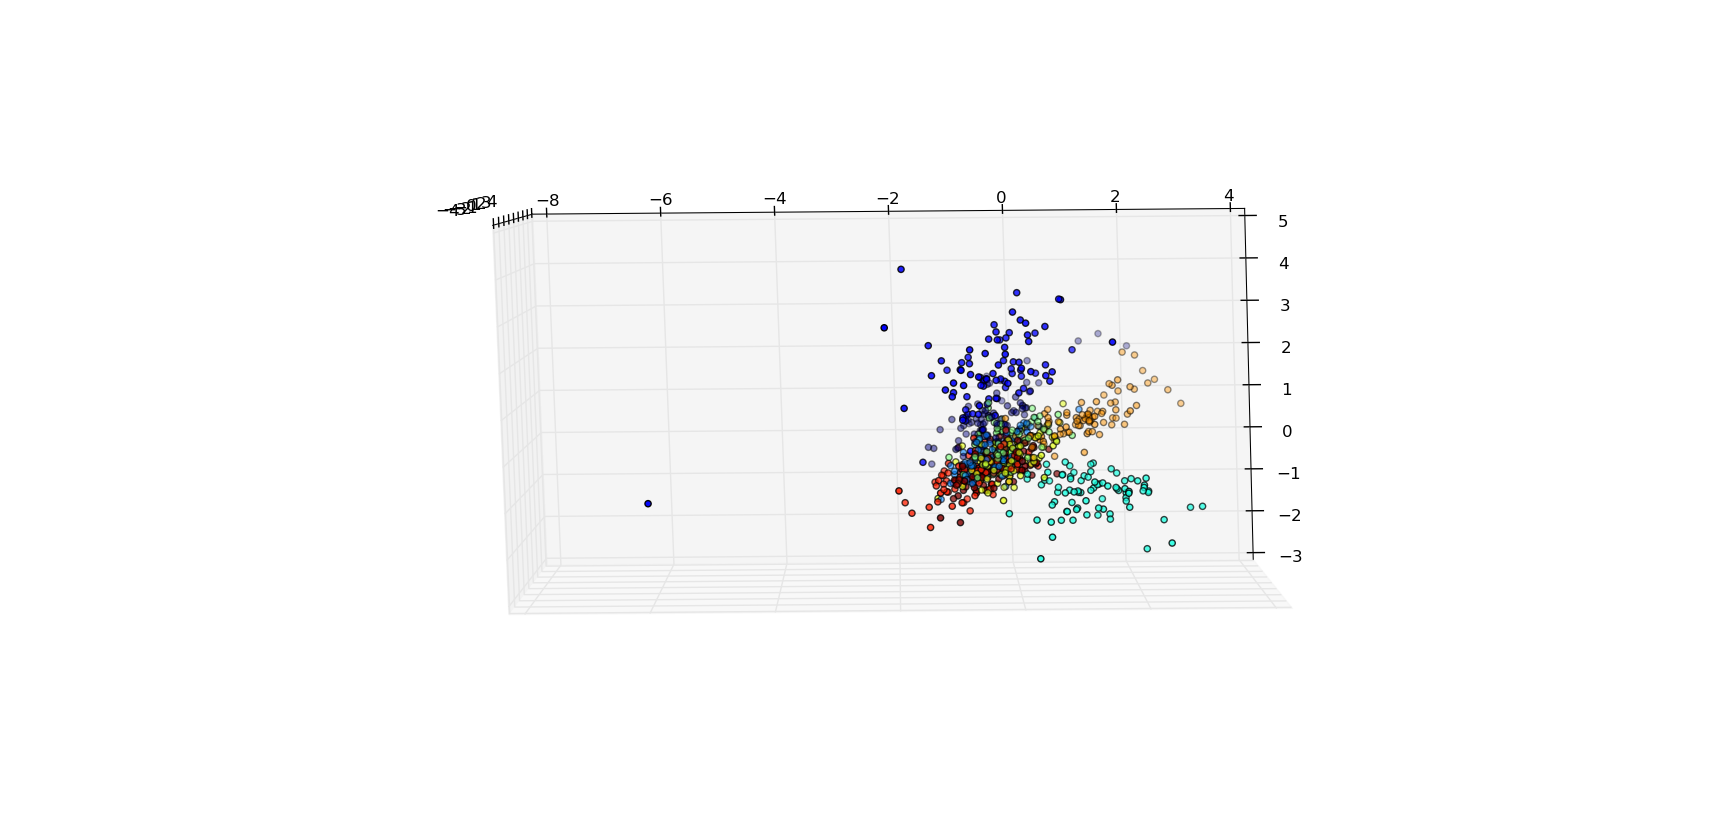
\includegraphics[width=1\linewidth, scale=1]{../img/ej1/oja/alt-oja_3salida_200ep_train_3.png}
%   \caption{Oja - 3 dimensiones - 200 épocas}
%   \label{fig:sub1}
% \end{subfigure}%
% \begin{subfigure}{.5\textwidth}
%   \centering
%   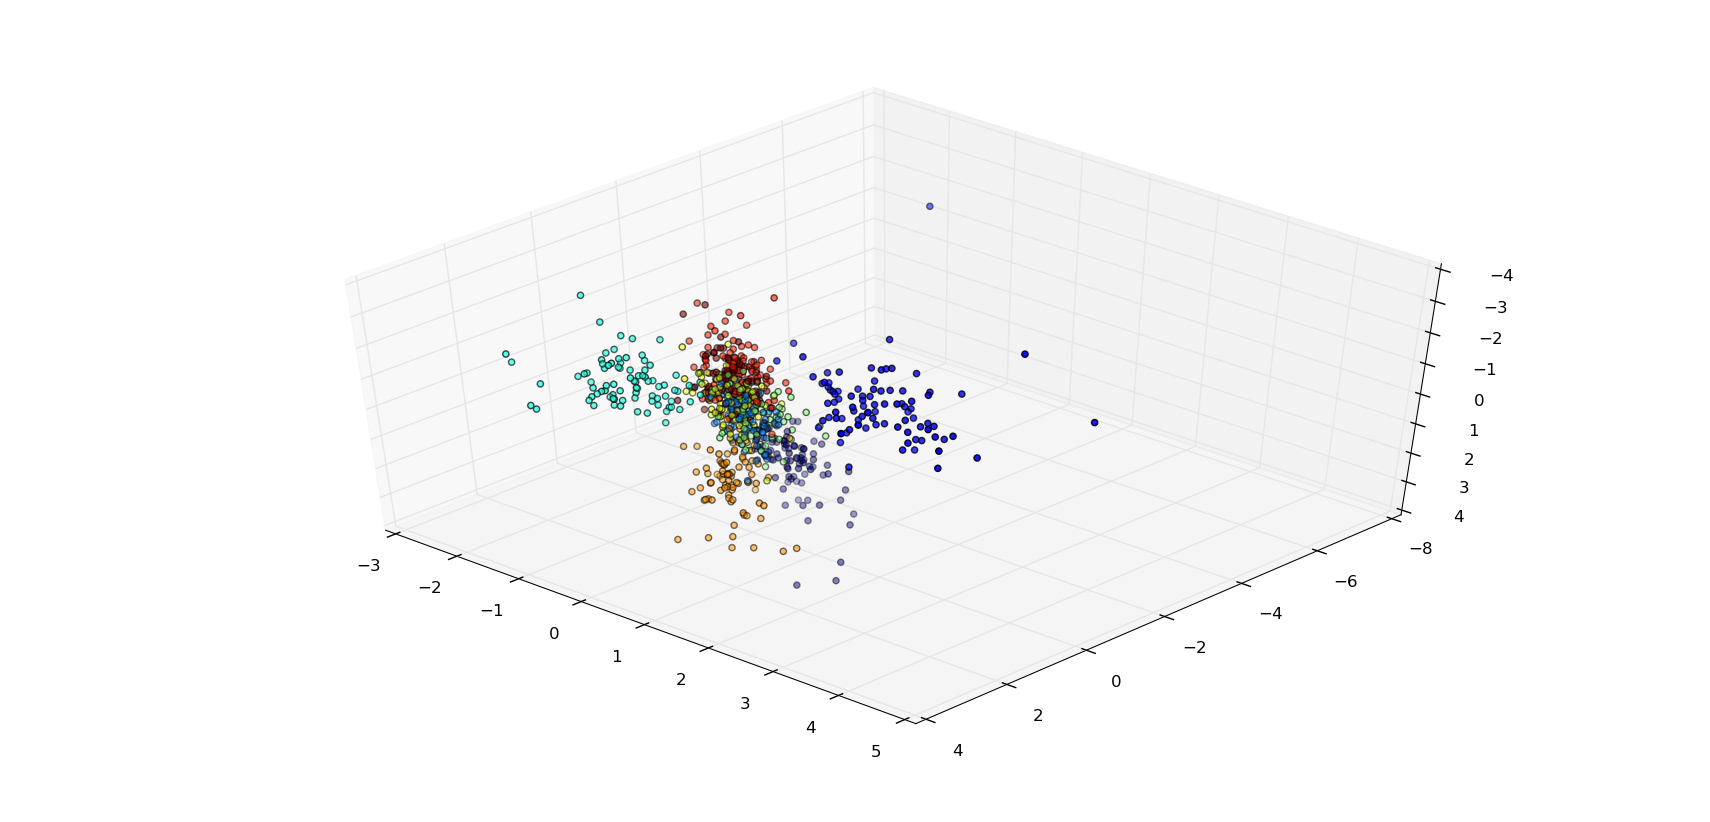
\includegraphics[width=1\linewidth, scale=1]{../img/ej1/oja/alt-oja_3salida_200ep_train_4.png}
%   \caption{Oja - 3 dimensiones - 200 épocas}
%   \label{fig:sub2}
% \end{subfigure}
% \end{figure}

\newpage
\subsection{Ejercicio 2}

\newpage
\section{Soluciones Óptimas Propuestas}

% Siguiendo las distintas conclusiones que fuimos formando a través de los experimentos, generamos una solución óptima para cada ejercicio del TP. Estas soluciones se encuentran codificadas en \textbf{solucion\_ej1.json} y \textbf{solucion\_ej2.json}.

% \subsection{Ejercicio 1}
% La solución del ejercicio 1 fue generada con los siguientes parámetros:

% \texttt{\$python script.py 1 -ep=250 -capas=10,10 -eta=0.05 -estop=0.1}

% La solución generó muy buenos resultados, obteniendo 94\% de efectividad con respecto a su dataset de testing.
% Con respecto al error final, así fue su evolución:

% \begin{figure}[h]
%   \begin{center}
%   \includegraphics[scale=0.50]{graficos/solucion_ej1.png}
%   \caption{Evolución del error a través del entrenamiento para la solución 1}
%   \end{center}
% \end{figure}

% Notamos que encontró valores muy bajos de error, con una curva bastante pronunciada a partir de la época 50. Observamos que el early stopping efectivamente entró en efecto, ya que cortó la ejecución antes de llegar al límite de épocas.\\

% En caso de querer cargar y probar esta red, ejecutar:

% \texttt{\$python script.py 1 -file=F -rda=solucion\_ej1.json -te=100 }

% donde \texttt{F} debe ser el path al archivo CSV que contenga el dataset seleccionado. El parámetro $te=100$ implica que se le ordena a la red predecir todos los resultados del dataset como testing y calcular su tasa de aciertos.

% \subsection{Ejercicio 2}
% La solución del ejercicio 2 fue generada con los siguientes parámetros:

% \texttt{\$python script.py 2 -ep=250 -capas=7 -estop=0.05}

% La solución generó resultados decentes, obteniendo 74\% de efectividad con respecto a su dataset de testing.\\
% Se nota una eficiencia menor a la de la solución del ejercicio 1.
% En la última figura podemos ver la evolución de las épocas y el error:

% \begin{figure}[h]
%   \begin{center}
%   \includegraphics[scale=0.50]{graficos/solucion_ej2.png}
%   \caption{Evolución del error a través del entrenamiento para la solución 2}
%   \end{center}
% \end{figure}

% \newpage

% Notamos en este caso un descenso más lento del error y un estancamiento final en la curva. No se llegó a aplicar la cláusula del early stopping.


% En caso de querer cargar y probar esta red, ejecutar:

% \texttt{\$python script.py 2 -file=F -rda=solucion\_ej2.json -te=100 }

% donde \texttt{F} debe ser el path al archivo CSV que contenga el dataset seleccionado.

% \newpage
\section{Conclusión}

% Como conclusión podemos ver que los distintos ejercicios y sus características obtuvieron diferentes resultados en los experimentos realizados.\\

% Notamos en ellos algunos fenómenos. En primer lugar, parecería que la cantidad óptima de neuronas en cada capa se acerca a la cantidad de atributos a procesar por la red. Esto se pudo observar en el experimento de cantidad de neuronas para cada ejercicios.\\
% En segundo lugar, apreciamos distintos efectos en la cantidad de épocas necesarias para llegar a buenos resultados. Cada ejercicio necesitó una cantidad diferente y muchos de los parámetros afectaron dicha cantidad, aumentándola ampliamente en varios casos.\\

% Algunos parámetros que pensamos que tendrían mayor efecto en los resultados fueron los de distribución de los pesos, momentum y en el caso del ejercicio 2, cantidad de capas. Nos sorprendió que finalmente la solución óptima no utilizara más estos factores.\\

% Aprendimos que parámetros como el early stopping, que de antemano parecía que si o si debería estar en nuestra solución, no nos dió resultados lo suficiente buenos 
% como para considerarlo como algo obligatorio a la hora de entrenar la red. Quizás esto fue porque la cantidad de épocas de nuestro entrenamiento no era la suficiente 
% como vimos anteriormente, y este relacionado también con que nuestro conjunto de datos es acotado, nuestra red pequeña y no se necesitan tantas épocas para entrenar.

% Vimos también que los parámetros adaptativos, como el learning rate, mejoran considerablemente soluciones como el entrenamiento batch o mini batch. Incluso, en el 
% entrenamiento batch, se puede llegar a conseguir una soluciones muy buenas si las épocas son suficientes con learning rate adaptativo.

% Finalmente observamos la naturaleza práctica de este tipo de problemas, en la cual muchos de las decisiones responden a experimentación y pruebas y no tanto a fundamentos teóricos o conceptuales.
